%
% teil3.tex -- Beispiel-File für Teil 3
%
% (c) 2020 Prof Dr Andreas Müller, Hochschule Rapperswil
%
% !TEX root = ../../buch.tex
% !TEX encoding = UTF-8
%
\subsection{Evaluation
\label{buch:paper:varalg:subsection:evaluation}}
\rhead{Evaluation}
Dieser Schritt befasst sich mit der Auswertung der einzelnen 
Kombinationen. In der Informatik wird die Liste genommen und 
die einzelnen Zusammenstellung wird berechnet.

Dafür wird die gleiche Formel \ref{eq:bruteforce_min_formula}, 
verwendet, die auch im Bruteforce-Methode Anwendung findet.

\begin{figure}
	\centering
	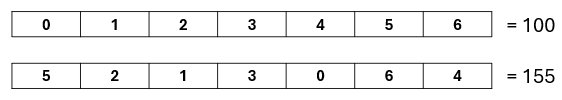
\includegraphics[width=0.8\textwidth]{
        papers/varalg/images/teil3/03GeneticStringCitiesResults.png
        }
	\caption{Beispiel eines genetischen Strings mit Ergebnissen}
	\label{fig:cities_genetic_string_results}
\end{figure}

